%!TEX ROOT = main.tex

\section{Final Project}

The purpose of the final project is to implement an efficient agent that can play and win Quarto. Quarto is a multi-player game where 2 players take turns placing pieces on a 4x4 board. The first player to place a piece that satisfies a winning condition wins the game. In my version of Quarto, I consider it to be a two-player game where my agent plays against a random opponent.

\subsection{My Strategy For Solving the Problem}

\subsubsection{Step 1: Implement and Tune Multiple Search Algorithms}

The following algorithms are implemented and the \textbf{best performing ones are combined to create a final, hybrid agent that balances speed and efficiency}:

\begin{itemize}
    \item \textbf{Random}: This agent randomly selects positions and pieces on the board. In the spirit of true randomness, it does not take into account the current state of the board.
    \item \textbf{Parameterized Hardcoded Play}: This agent has a set of fixed rules, where it attempts to build a line of like pieces. Where it cannot, it attempts
    \item \textbf{Deep Q-Learning}: This agent uses a deep neural network to approximate the Q-function. It uses a replay buffer to store the experience tuples and uses a target network to stabilize the training process. The agent uses an epsilon-greedy policy to balance exploration and exploitation. The input to the linear network is a flatten list of 1x16 pieces based on the current board composition, while the input to the convolutional neural network is a 4x4x4 board composition.
    \item \textbf{Q-Learning (Temporal Difference Learning)}: This agent uses a Q-table to store the Q-values. It uses a replay buffer to store the experience tuples and uses a target network to stabilize the training process. The agent uses an epsilon-greedy policy to balance exploration and exploitation. A custom OpenAI Gym environment is created to make training easier.
    \item \textbf{Monte Carlo Tree Search}: This agent uses a Monte Carlo Tree Search algorithm to select the best move. It uses a UCB1 formula to select the best child node at each iteration.
    \item \textbf{QL-MCTS}: This algorithm uses a Q-table as it's base and uses a rolled out Monte Carlo Search Tree for a more efficient search. When a state cannot be found in the Q-table, the agent once again goes to the Monte Carlo Tree Search algorithm to find the best move.
\end{itemize}

The following algorithms failed, producing only a near-random win rate after several hours of training:

\begin{enumerate}
    \item \textbf{Pure Q-Learning}: This agent stores moves made in a Q-table and could not perform feasibly in a test environment even after hours of training, growing it's Q-table and implementing board symmetries.
    \item \textbf{Deep Q-Learning (Linear and Convolutional Neural Network)}: In this approach, I train a 4-layer deep neural network to predict the Q-values of a given state. Despite several hours of training and hyperparameter tuning (changing the number of layers, optimiser, learning rate), the agent could only reach a 60\% win rate in its best attempt. I also tried a convolutional neural network to feed the entire board composition as a 4x4x4 input (third dimension is the piece attribute), but training was far too slow.  \\ \\
    \textbf{Best Model Depth and Configuration}: 4-layer linear neural network of node sizes (24, 48, 96, 192), Huber Loss, Adam Optimiser, Learning Rate of 0.001

    \begin{equation*}
        L_{\delta}=
    \left\{\begin{matrix}
        \frac{1}{2}(y - \hat{y})^{2} & if \left | (y - \hat{y})  \right | < \delta\\
        \delta ((y - \hat{y}) - \frac1 2 \delta) & otherwise
    \end{matrix}\right.
    \end{equation*}

    \textbf{Best Results}: 55\% win rate after 1000 episodes of training \\ \\
    Training time was too slow and convergence could not be reached in a reasonable time. I had already spent multiple weeks on this approach to no fruition. If I had more computational resources, I would train this model for much longer to see if true convergence can be reached.
\end{enumerate}

\subsubsection{Step 2: Analysing the Algorithms}

The best performing algorithms were the hardcoded agent and Monte Carlo Tree Search, that produced high win rates (>80\%). However, important observations for each strategy are:

\begin{itemize}
    \item \textbf{Hardcoded Agent}: This agent is fast, but it is not efficient. It is only able to win the game if it is able to build a line of like pieces. If it cannot, it will return to a series of random moves that may/may not win the game.
    \item \textbf{Monte Carlo Tree Search}: MCTS rolls out and computes the reward from each board state but it is slow. It appears that it is not worth using at the start of the game, where a terminal state is quite distant from the current board position. Furthermore, a major problem with MCTS is the tree size, which grows exponentially with game progression. \textbf{This makes rolling out at each subsequent move slower than the previous rollout.} \\
\end{itemize}

Solution: Instead of keeping an extremely large tree, we record the result of each \textit{state, action} pair in a Q-table, updated using Temporal Difference Learning and the Bellman equation. On the off chance that a past board state is encountered, the Q-table can be used to find the best corresponding action, instead of having to iterate through the entire tree. I call this the \textbf{QL-MCTS} algorithm, with inspiration from Wang et al. (2018) approach to Monte-Carlo Q-Learning. QL-MCTS works by:

\begin{itemize}
    \item When training the Q-learning agent, use MCTS to find the best moves instead of using random in the epsilon-greedy policy.
    \item If the agent is called and a particular state-action combination is not present in the Q-table, go to MCTS to find the best move.
\end{itemize}

\subsubsection{Step 3: Implementing the Hybrid Agent}

Using the best performing algorithms, I created a hybrid agent that works in 3 phases. First, to get the game started, it will make random moves. After this, it will switch to a hardcoded strategy where it will attempt to computationally build lines of similar pieces. Finally, it will leverage the QL-MCTS algorithm to find the best moves and win the game. Since QL-MCTS is slow, it is kept as the final phase. This approach is shown in Figure \ref{fig:hybrid-agent}, and is a balance between speed and efficiency.

\begin{figure}
    \centering
    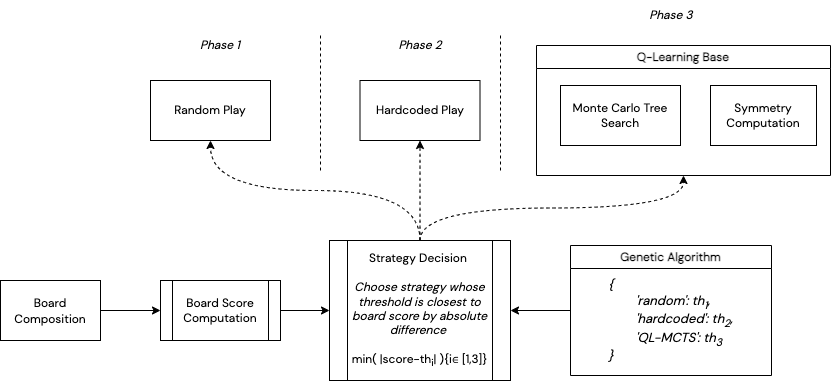
\includegraphics[width=0.9\textwidth]{images/methodology.drawio.png}
    \caption{Hybrid Agent}
    \label{fig:hybrid-agent}
\end{figure}

The main question is when to switch between the algorithms. The intuition is that the switch depends on the change of the board composition. We represent this numerically through a board score, that is essentially a sum of couplets and triplets.

\begin{equation*}
    couples + 2 * triplets
\end{equation*}

The range of values for scores $\in [0, 16]$. We try to generate score thresholds to switch between the 3 strategies using a genetic algorithm. An example of a genome is shown in Figure \ref{json-example}.

\begin{listing}
    \begin{minted}{json}
    {
        "random": 3,
        "hardcoded" : 5,
        "ql-mcts" : 8
    }
    \end{minted}
    \caption{Genome Example}
    \label{json-example}
    \end{listing}

We train the genetic algorithm for 1000 generations and a population size of 100, to find the best genome and submit these as the thresholds for the hybrid agent.

Once the final thresholds are found, we find the strategy whose threshold has the smallest absolute difference with the current board score. The minimisation formula is:

\begin{equation*}
    \text{strategy} = \min_{i=1}^{3} \left| \text{threshold}_i - \text{board score} \right|
\end{equation*}

\subsection{Code}

The code for this project is available on GitHub at \url{https://github.com/sidharrth2002/ci-quarto-sidharrth}.

\subsection{Acknowledgements}

Throughout this project, I have discussed with Diego Gasco. We started the project by discussing ideas for strategies.

\begin{itemize}
    \item After I tried to get a working Deep Q-Network and realised that it wasn't converging in reasonable time, we discussed the possibility of using some tree search algorithm. It was Diego who suggested MCTS.
    \item When realising that MCTS can be quite slow towards the end of the game, I suggested building a hybrid QL-MCTS player that would use a base Q-table to remember the best moves so the quadratically complex tree wouldn't need to store so many nodes.
    \item We later built a hardcoded agent using different rules and realised that it performed very well, and was quick to make a move.
    \item We then decided to combine everything we did into a hybrid agent that would switch between strategies depending on the board score.
    \item Diego suggested a good scoring function. He also suggested that a genetic algorithm could be used for this.
    \item I suggested finding score thresholds to switch between strategies using a genetic algorithm.
\end{itemize}

While we follow the same hybrid strategy, our code is quite different, apart from a few shared utility functions.
